% !TEX root = ../main.tex

% Background section

\newtheorem{definition}{Definition}
\newtheorem{lemma}{Lemma}

\section{Background}

By our nature of intelligence being, we have the intuitive motivation of ··learning". The basic mechanism of statistical learning is the ability for humans and other animals to extract statistical regularities from the world around them to learn about the environment. In this project, we will explore the learnability of a hypothesis class through a foundation algorithm in the universal learning theory: Empirical Risk Minimization by walking through the problem setting and theory construction\\

\subsection{General Learning Problem Setting}
There are many classic learning problems utilized in the real life, such as classifying set of emails into spam/not spam, optimal portfolio selection, and weather forecasting. In the basic statistical setting, a learning problem is characterized by the following components: 
\begin{itemize} 
    \item \textbf{Domain Set $\chi$}: A arbitrary set $\chi$ that is the set of objects that we wish to classify or label. Mostly we concerned with the case where $\chi = \mathbb{R}^{d}$ or $\chi = \{0,1\}^{d}$, in which each object that we want to label is characterized by $d$ real numbers. The attributes are referred to as features.
    \item \textbf{Label Set $\mathcal{Y}$}: The set $\mathcal{Y}$ describe the labels, which will be used for learners to assign for each $x \in \mathcal{X}$ a label $y \in \mathcal{Y}$.
\end{itemize}
We assumes that there exists a distribution $\mathcal{D}$ over $\mathcal{X} \times \mathcal{Y}$ that generates labeled examples. For example, pairs $(x,y) \in \mathcal{X} \times \mathcal{Y}$.\\

\subsection{Elements of A statistical Learning Model}
A statistical learning model usually consists of the following elements:
\begin{itemize}
    \item \textbf{Input} A set of labeled examples in the training set  $S={(x_{1},y_{1}),...,(x_{m},y_{m})} \subseteq \mathcal{X} \times \mathcal{Y}$. This is the input that is known, and we denote the size of training set as $m$.
    \item \textbf{Output}: A prediction rule/hypothes is $ \mathcal{H}: h: \mathcal{X} \rightarrow \mathcal{Y} $, which turns unlabeled samples to labels.
    \item \textbf{Data}: As we mentioned above,  we assumes that exists an unknown distribution $\mathcal{D} $ over $\mathcal{X}$ and the label is generated by some mapping $f : \mathcal{X} \rightarrow \mathcal{Y}$. $S$ is created by iid samples from $\mathcal{D}$, and they are classified by $f$.
    
    \item \textbf{Performance metric}: The risk/generalization error. Given a distribution $D$ over $\mathcal{X}$, the learner is required to give a hypothesis $h : \mathcal{X} \rightarrow \mathcal{Y}$. This functions is called predictor or a classifier. The quality of each hypothesis $h \subseteq \mathcal{H}$ is measured by its $\operatorname{err}(h)=\mathbb{P}_{x \sim D}[h(x) \neq f(x)]=\mathbb{E}_{x \sim D}[|h(x)-f(x)|]$. Ideally, we are interested in picking $h \in \mathcal{H}$ whose risk is as close as possible to $\inf_{h \in \mathcal{H}} \operatorname{err}(h)$. Since the distribution $\mathcal{D}$ is unknown, we cannot do this directly, but we can rely on our empirical training sample $\mathcal{S}$. Generally, we expect the approximation to get better performance with larger sample size. A learning rule that allow us to choose such $h$ are said to be consistent. \cite{Hazan}\\
\end{itemize}   
    
\subsection {The Probably Approximately Correct Learning (PAC)}
    We will utilize the concept of the PAC learning when exploring the learnability of hypothesis class. We start by proposing a simple example. Let our domain set $\mathcal{X}$ as a line, by placing a threshold $\theta \in \mathbb{R}$ on the line, we have
    \[
  h_{\theta}(x) =
  \begin{cases}
                                   y_{i} & \text{if $x$ in the left hand side of $\theta$} \\
                                   0 & \text{if $x$ in the right hand side of $\theta$} 
  \end{cases}
\]
We can easily observe that the data following a uniform distribution $\mathcal{D}$, however, the information of distribution $\mathcal{D}$ is blind to our algorithm. Our goal for the algorithm is to learn the threshold $r$ that can classify the data points into two classes with error less than a given constant $\varepsilon$. In this situation, there are a few facts that we need to aware. One is that, with a finite empirical training set, it is almost impossible to achieve error-free classification. Therefore, we will turn to pursue an approximately correct output. The other one would be it is possible that a correct output is only probably correct instead of being truly correct, because there exist a situation in which the training set is not representative of the whole data. 


\begin{definition} (The PAC Learning)
    An algorithm $\mathcal{L}$ PAC learns a unknown $f$ if $\forall \mathcal{D}$ $\exists \varepsilon>0$ and $\exists \delta >0$. Let $h_{\mathcal{L}}$ be the function that $\mathcal{L}$ output, then 
    \begin{equation*}
        P(\operatorname{err}(h_{\mathcal{L}}) \leq \varepsilon) \geq 1 - \delta
    \end{equation*}
\end{definition}
\noindent An extremely important lemma that assists with the PAC learning is about the size the training set that can achieve the PAC learning. 

\begin{lemma}
To achieve a PAC guarantee, the following condition holds true for the sample size $m$:
\begin{equation*}
    m \leq \frac{1}{\varepsilon}\log(\frac{2}{\delta})
\end{equation*}
\end{lemma}

\begin{proof}
Pranjal Awasthi presents an detailed solution shown as follows.\cite{Awasthi:1} We scan the training samples from left to right and put a threshold $r$ anywhere in the region where there is a change in label like (A) in figure 1. Let the sample size as $m$, if $\theta$ lies in the region $R$, then we can be confident that $\operatorname{err}(h) \leq \varepsilon$. A necessary condition is that the training set must have at least 2 examples from the region $R$ with one with each class respectively. Since the probability of a single data point in the training set is not within $(\theta - \varepsilon, \theta)$ is less or equal to $1-\varepsilon$, and the probability of that is not within $(\theta, \theta + \varepsilon)$ is also less or equal to $1-\varepsilon$. Because of independence of each data point, we won't see at least one example from both regions is upper bounded by $2(1-\varepsilon)^{m}$. To achieve the PAC learning, the sample size $m$ must satisfy the following condition:
\begin{equation*}
    \begin{aligned}
        2(1-\varepsilon)^{m} & \leq \delta \\
        \rightarrow m &\leq \frac{1}{\varepsilon}\log(\frac{2}{\delta})
    \end{aligned}
\end{equation*}


\begin{figure}[h] 
    \centering
    \subfloat[A]{%
        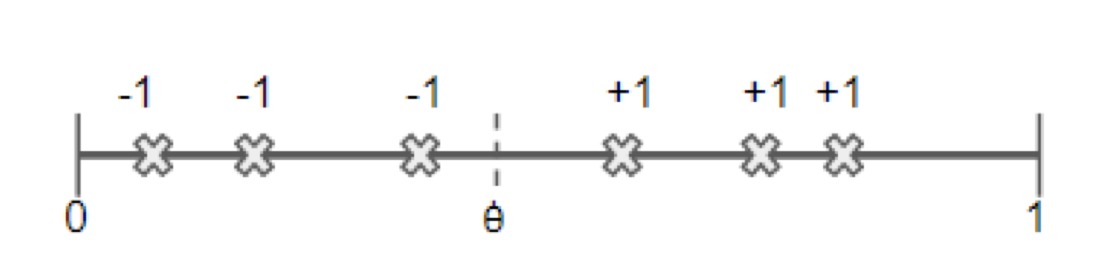
\includegraphics[width=0.3\textwidth]{misc/figure1.png}%
        \label{fig:a}%
        }%
    \hfill%
    \subfloat[B]{%
        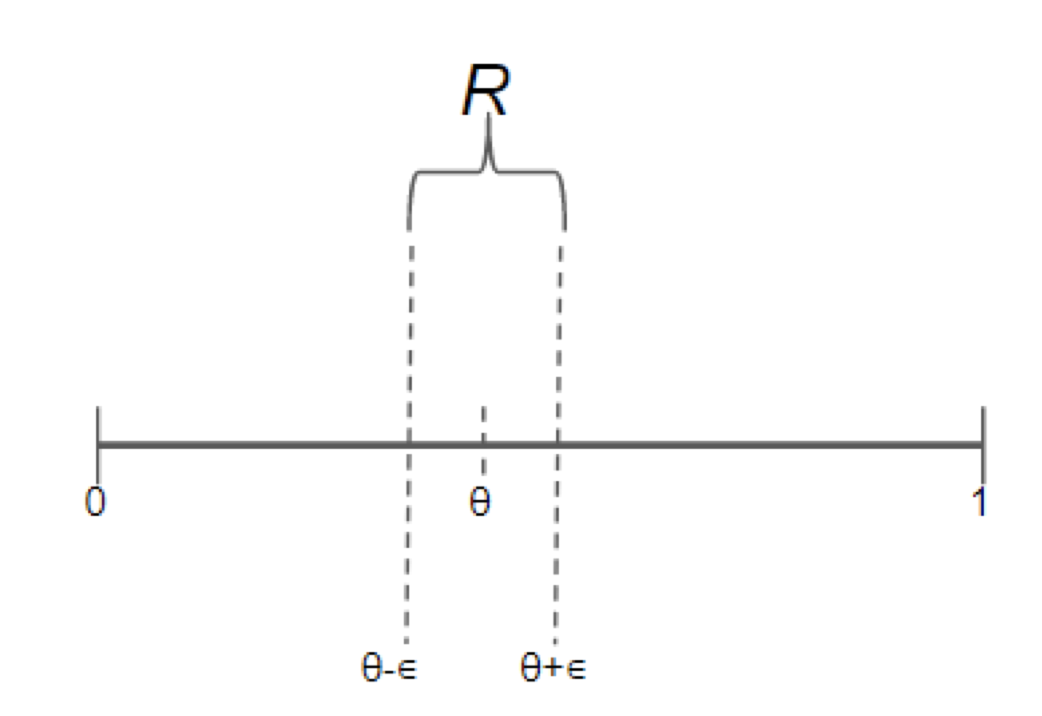
\includegraphics[width=0.3\textwidth]{misc/figure2.png}%
        \label{fig:b}%
        }%
    \caption{PAC Learning}
\end{figure}
\end{proof}

\newpage
   
\subsection{The Empirical Risk Minimization}
Recalling from the previous two-class example, we have the prior knowledge that the data is generated form a uniform distribution. Therefore, we roughly have an initial judge of how the threshold function will look like, which is impossible for most situations in practice. Therefore, we are interested in finding an generic algorithm that fits any types of functions. Our objective is to obtain a hypothesis that minimizes the empirical error on the training set where we have a finite number of hypotheses, and at least one of which has zero expected risk. 

\begin{definition}(\textbf{Empirical Risk Minimization})
The empirical risk minimization algorithm $h_{ERM} : X \rightarrow Y$ is the classifier that achieves the minimum error on the test set $S$. Suppose $h* \in \mathcal{H}$ is the true function that describes the data (error euqal $0$), where $\mathcal{H}$ is finite. Given a training set $\mathcal{S} = \{ s_{1},...,s_{m}\} = \{(x_{1},y_{i}),...,(x_{m},y_{m}) \}$, the function returned by the ERM algorithm will be

\begin{equation*}
    h_{ERM} = \operatorname{argmin}_{h \in \mathcal{H}} \operatorname{err}_{\mathcal{S}}(h)
\end{equation*}
where $\operatorname{err}_{\mathcal{S}}(h)$ is the fraction of incorrect classification that $h$ makes on the training set.
Namely, $h_{ERM}$ is the optimal function that produces the lowest error on the training set. 
\end{definition}
